\documentclass[12pt,]{article}
\usepackage{lmodern}
\usepackage{amssymb,amsmath}
\usepackage{ifxetex,ifluatex}
\usepackage{fixltx2e} % provides \textsubscript
\ifnum 0\ifxetex 1\fi\ifluatex 1\fi=0 % if pdftex
  \usepackage[T1]{fontenc}
  \usepackage[utf8]{inputenc}
\else % if luatex or xelatex
  \ifxetex
    \usepackage{mathspec}
    \usepackage{xltxtra,xunicode}
  \else
    \usepackage{fontspec}
  \fi
  \defaultfontfeatures{Mapping=tex-text,Scale=MatchLowercase}
  \newcommand{\euro}{€}
    \setmainfont{Palatino}
    \setsansfont{Century Gothic}
    \setmonofont[Mapping=tex-ansi]{Consolas}
\fi
% use upquote if available, for straight quotes in verbatim environments
\IfFileExists{upquote.sty}{\usepackage{upquote}}{}
% use microtype if available
\IfFileExists{microtype.sty}{%
\usepackage{microtype}
\UseMicrotypeSet[protrusion]{basicmath} % disable protrusion for tt fonts
}{}
\ifxetex
  \usepackage[setpagesize=false, % page size defined by xetex
              unicode=false, % unicode breaks when used with xetex
              xetex]{hyperref}
\else
  \usepackage[unicode=true]{hyperref}
\fi
\hypersetup{breaklinks=true,
            bookmarks=true,
            pdfauthor={Amin Meyghani},
            pdftitle={Introduction to Angular 2},
            colorlinks=true,
            citecolor=blue,
            urlcolor=blue,
            linkcolor=magenta,
            pdfborder={0 0 0}}
\urlstyle{same}  % don't use monospace font for urls
\usepackage{fancyhdr}
\pagestyle{fancy}
\pagenumbering{arabic}
\lhead{\itshape Introduction to Angular 2}
\chead{}
\rhead{\itshape{\nouppercase{\leftmark}}}
\lfoot{}
\cfoot{}
\rfoot{\thepage}
\usepackage{color}
\usepackage{fancyvrb}
\newcommand{\VerbBar}{|}
\newcommand{\VERB}{\Verb[commandchars=\\\{\}]}
\DefineVerbatimEnvironment{Highlighting}{Verbatim}{commandchars=\\\{\}}
% Add ',fontsize=\small' for more characters per line
\newenvironment{Shaded}{}{}
\newcommand{\KeywordTok}[1]{\textcolor[rgb]{0.00,0.00,1.00}{{#1}}}
\newcommand{\DataTypeTok}[1]{{#1}}
\newcommand{\DecValTok}[1]{{#1}}
\newcommand{\BaseNTok}[1]{{#1}}
\newcommand{\FloatTok}[1]{{#1}}
\newcommand{\ConstantTok}[1]{{#1}}
\newcommand{\CharTok}[1]{\textcolor[rgb]{0.00,0.50,0.50}{{#1}}}
\newcommand{\SpecialCharTok}[1]{\textcolor[rgb]{0.00,0.50,0.50}{{#1}}}
\newcommand{\StringTok}[1]{\textcolor[rgb]{0.00,0.50,0.50}{{#1}}}
\newcommand{\VerbatimStringTok}[1]{\textcolor[rgb]{0.00,0.50,0.50}{{#1}}}
\newcommand{\SpecialStringTok}[1]{\textcolor[rgb]{0.00,0.50,0.50}{{#1}}}
\newcommand{\ImportTok}[1]{{#1}}
\newcommand{\CommentTok}[1]{\textcolor[rgb]{0.00,0.50,0.00}{{#1}}}
\newcommand{\DocumentationTok}[1]{\textcolor[rgb]{0.00,0.50,0.00}{{#1}}}
\newcommand{\AnnotationTok}[1]{\textcolor[rgb]{0.00,0.50,0.00}{{#1}}}
\newcommand{\CommentVarTok}[1]{\textcolor[rgb]{0.00,0.50,0.00}{{#1}}}
\newcommand{\OtherTok}[1]{\textcolor[rgb]{1.00,0.25,0.00}{{#1}}}
\newcommand{\FunctionTok}[1]{{#1}}
\newcommand{\VariableTok}[1]{{#1}}
\newcommand{\ControlFlowTok}[1]{\textcolor[rgb]{0.00,0.00,1.00}{{#1}}}
\newcommand{\OperatorTok}[1]{{#1}}
\newcommand{\BuiltInTok}[1]{{#1}}
\newcommand{\ExtensionTok}[1]{{#1}}
\newcommand{\PreprocessorTok}[1]{\textcolor[rgb]{1.00,0.25,0.00}{{#1}}}
\newcommand{\AttributeTok}[1]{{#1}}
\newcommand{\RegionMarkerTok}[1]{{#1}}
\newcommand{\InformationTok}[1]{\textcolor[rgb]{0.00,0.50,0.00}{{#1}}}
\newcommand{\WarningTok}[1]{\textcolor[rgb]{0.00,0.50,0.00}{\textbf{{#1}}}}
\newcommand{\AlertTok}[1]{\textcolor[rgb]{1.00,0.00,0.00}{{#1}}}
\newcommand{\ErrorTok}[1]{\textcolor[rgb]{1.00,0.00,0.00}{\textbf{{#1}}}}
\newcommand{\NormalTok}[1]{{#1}}
\usepackage{graphicx,grffile}
\makeatletter
\def\maxwidth{\ifdim\Gin@nat@width>\linewidth\linewidth\else\Gin@nat@width\fi}
\def\maxheight{\ifdim\Gin@nat@height>\textheight\textheight\else\Gin@nat@height\fi}
\makeatother
% Scale images if necessary, so that they will not overflow the page
% margins by default, and it is still possible to overwrite the defaults
% using explicit options in \includegraphics[width, height, ...]{}
\setkeys{Gin}{width=\maxwidth,height=\maxheight,keepaspectratio}
\setlength{\parindent}{0pt}
\setlength{\parskip}{6pt plus 2pt minus 1pt}
\setlength{\emergencystretch}{3em}  % prevent overfull lines
\providecommand{\tightlist}{%
  \setlength{\itemsep}{0pt}\setlength{\parskip}{0pt}}
\setcounter{secnumdepth}{5}

\title{Introduction to Angular 2}
\author{Amin Meyghani}
\date{}

% Redefines (sub)paragraphs to behave more like sections
\ifx\paragraph\undefined\else
\let\oldparagraph\paragraph
\renewcommand{\paragraph}[1]{\oldparagraph{#1}\mbox{}}
\fi
\ifx\subparagraph\undefined\else
\let\oldsubparagraph\subparagraph
\renewcommand{\subparagraph}[1]{\oldsubparagraph{#1}\mbox{}}
\fi

\begin{document}
\maketitle

{
\hypersetup{linkcolor=black}
\setcounter{tocdepth}{5}
\tableofcontents
}
\section{Notes}\label{notes}

\begin{itemize}
\item
  The book assumes that you are working in a Unix-like environment. If
  you are on Windows you can use \href{https://www.cygwin.com/}{Cygwin}
  so that you can follow along with the bash terminal commands.
\item
  All the project files for the book are hosted on github:
  \url{https://github.com/st32lth/angular2-intro}. You can clone the
  repository and check out the project files. Throughout the book, you
  will see references to the project files. Those refer to this
  repository. For example,
  \texttt{angular2-intro/project-files/hello-angular} refers to the
  \texttt{hello-angular} folder inside the \texttt{project-files}
  folder.
\item
  Make sure you have \texttt{git} installed on your machine. That is,
  make sure you get an output for \texttt{git\ -\/-version}.
\item
  The book assumes that you have a working knowledge of JavaScript and
  Angular 1.x
\item
  Node is heavily used throughout the book. Make sure that you follow
  the ``Node'' chapter to install Node and set permissions correctly.
\item
  All the keyboard shortcuts are mac-based. But if you are using a
  non-mac machine, you can almost always replace \texttt{command} with
  \texttt{ctrl} and you should be good. For example, if you a see a
  shortcut like \texttt{command\ +\ shift\ +\ b}, you can use
  \texttt{ctrl\ +\ shift\ +\ b} where \texttt{ctrl} is obviously the
  \texttt{control} key.
\end{itemize}

\section{Installing Node}\label{installing-node}

You can use \href{https://github.com/creationix/nvm}{nvm} to install and
manage Node on your machine. Copy the install script and run it:

\begin{Shaded}
\begin{Highlighting}[numbers=left,,]
\KeywordTok{curl} \NormalTok{-o- https://raw.githubusercontent.com/creationix/nvm/v0.30.1/install.sh }\KeywordTok{|} \KeywordTok{bash}
\end{Highlighting}
\end{Shaded}

After that, make a new terminal window and make sure that it is
installed, by running:

\begin{Shaded}
\begin{Highlighting}[numbers=left,,]
\KeywordTok{nvm} \NormalTok{--help}
\end{Highlighting}
\end{Shaded}

Now you can use \texttt{nvm} to install Node \texttt{0.12.9} by running:

\begin{Shaded}
\begin{Highlighting}[numbers=left,,]
\KeywordTok{nvm} \NormalTok{install 0.12.9}
\end{Highlighting}
\end{Shaded}

After that, nvm is going to load version 0.12.9 automatically. If it
doesn't, you can load it in the current shell, with:

\begin{Shaded}
\begin{Highlighting}[numbers=left,,]
\KeywordTok{nvm} \NormalTok{use 0.12.9}
\end{Highlighting}
\end{Shaded}

Note that you can load any node version in the current shell with
\texttt{nvm\ use\ 0.x.y} after installing that version.

Also note that if you want to make \texttt{0.12.9} the default Node
version on your machine, you can do so by running the following:

\begin{Shaded}
\begin{Highlighting}[numbers=left,,]
\KeywordTok{nvm} \NormalTok{alias default 0.12.9}
\end{Highlighting}
\end{Shaded}

Then you can verify that it is the default version by making a new
terminal window and typing \texttt{node\ -v}.

\subsection{Permissions}\label{permissions}

Never use \texttt{sudo} to install packages, never do
\texttt{sudo\ npm\ install\ \textless{}package\textgreater{}}. If you
get permission errors while installing without \texttt{sudo}, you can
own the folders instead. So for example, if you get an error like:

\begin{Shaded}
\begin{Highlighting}[numbers=left,,]
\KeywordTok{Error}\NormalTok{: EACCES, mkdir }\StringTok{'/usr/local'}
\end{Highlighting}
\end{Shaded}

you can own the folder with:

\begin{Shaded}
\begin{Highlighting}[numbers=left,,]
\KeywordTok{sudo} \NormalTok{chown -R }\KeywordTok{`whoami`} \NormalTok{/usr/local}
\end{Highlighting}
\end{Shaded}

You can own folders until Node doesn't complain.

\subsection{\texorpdfstring{Installing
\texttt{live-server}}{Installing live-server}}\label{installing-live-server}

Install a package to verify that node is installed and everything is
wired up correctly. We are going to use \texttt{live-server} through the
book. So let's install that with:

\begin{Shaded}
\begin{Highlighting}[numbers=left,,]
\KeywordTok{npm} \NormalTok{i -g live-server}
\end{Highlighting}
\end{Shaded}

Then, you should be able to run \texttt{live-server} in any folder to
serve the content of that folder:

\begin{Shaded}
\begin{Highlighting}[numbers=left,,]
\KeywordTok{mdkir} \NormalTok{~/Desktop/sample }\KeywordTok{&&} \KeywordTok{cd} \OtherTok{$_}
\KeywordTok{live-server} \NormalTok{.}
\end{Highlighting}
\end{Shaded}

\section{Visual Studio Code}\label{visual-studio-code}

Visual Studio Code is a good IDE for developing web apps. In this
chapter we will look at installing and configuring VSCode.

\subsection{Visual Studio Code Basics}\label{visual-studio-code-basics}

\begin{itemize}
\item
  Install Visual Studio Code from: \url{https://code.visualstudio.com/}
\item
  You can open new projects by going to the
  \texttt{File\ \textgreater{}\ Open} tag, to etierh open a folder
  containing your project or a single file
\item
  Some useful keyboard shortcuts are:

  \begin{itemize}
  \tightlist
  \item
    \texttt{command\ +\ b}: to close/open the file navigator
  \item
    \texttt{command\ +\ shift\ +\ p}: to open the prompt
  \end{itemize}
\item
  To install extensions open the prompt with
  \texttt{command\ +\ shift\ +\ p} and type:

\begin{verbatim}
> install extension
\end{verbatim}
\item
  You can change the keyboard shortcuts settings from
  \texttt{Preferences\ \textgreater{}\ Keyboard\ Shortcuts}. Open the
  settings and then you can add your own shortcuts:

\begin{verbatim}
// Place your key bindings in this file to overwrite the defaults
[
  {
    "key": "cmd+t",
    "command": "workbench.action.quickOpen"
  },
  {
    "key": "shift+cmd+r",
    "command": "editor.action.format",
    "when": "editorTextFocus"
  }
]
\end{verbatim}
\end{itemize}

\subsection{Setting up VSCode for
TypeScript}\label{setting-up-vscode-for-typescript}

In this section we are going to set up Visual Studio Code for
TypeScript. The project files for this chapter are in
\textbf{\href{https://github.com/st32lth/angular2-intro/tree/master/project-files/vscode-demo}{\texttt{angular2-intro/project-files/vscode-demo}}}.
You can either follow along or check out the folder to see the final
result.

\subsubsection{Installing TypeScript}\label{installing-typescript}

Before anything, we need to install the TypeScript compiler. You can
install the TypeScript compiler with npm:

\begin{Shaded}
\begin{Highlighting}[numbers=left,,]
\KeywordTok{npm} \NormalTok{i typescript -g}
\end{Highlighting}
\end{Shaded}

Then to verify that it is installed, run \texttt{tsc\ -v} to see the
version of the compiler. You will get an output like this:

\begin{verbatim}
message TS6029: Version 1.7.5
\end{verbatim}

In addition to the compiler, we also need to install the TypeScript
Definition manager for DefinitelyTyped (tsd). You can install tsd with:

\begin{Shaded}
\begin{Highlighting}[numbers=left,,]
\KeywordTok{npm} \NormalTok{i tsd -g}
\end{Highlighting}
\end{Shaded}

Using TSD, you can search and install TypeScript definition files
directly from the community driven DefinitelyTyped repository. To verify
that tsd is installed, run tsd with the \texttt{version} flag:

\begin{Shaded}
\begin{Highlighting}[numbers=left,,]
\KeywordTok{tsd} \NormalTok{--version}
\end{Highlighting}
\end{Shaded}

You should get an output like this:

\begin{verbatim}
>> tsd 0.6.5
\end{verbatim}

After \texttt{tsd} and \texttt{tsc} are installed, we can compile a
hello world program:

make a file called \texttt{hello.ts} on your desktop:

\begin{Shaded}
\begin{Highlighting}[numbers=left,,]
\KeywordTok{touch} \NormalTok{~/Desktop/hello.ts}
\end{Highlighting}
\end{Shaded}

Then, put some TypeScript code in the file:

\begin{Shaded}
\begin{Highlighting}[numbers=left,,]
\KeywordTok{echo} \StringTok{"const adder = (a: number, b: number): number => a + b;"} \KeywordTok{>} \NormalTok{~/Desktop/hello.ts}
\end{Highlighting}
\end{Shaded}

Then you can compile the file to JavaScript:

\begin{Shaded}
\begin{Highlighting}[numbers=left,,]
\KeywordTok{tsc} \NormalTok{~/Desktop/hello.ts}
\end{Highlighting}
\end{Shaded}

It should output a file in \texttt{Desktop/hello.js}:

\begin{Shaded}
\begin{Highlighting}[numbers=left,,]
\KeywordTok{var} \NormalTok{adder }\OperatorTok{=} \KeywordTok{function} \NormalTok{(a}\OperatorTok{,} \NormalTok{b) }\OperatorTok{\{} \ControlFlowTok{return} \NormalTok{a }\OperatorTok{+} \NormalTok{b}\OperatorTok{;} \OperatorTok{\};}
\end{Highlighting}
\end{Shaded}

Now that your TypeScript compiler setup, we can move on to configuring
Visual Studio Code.

\subsubsection{Add VSCode
Configurations}\label{add-vscode-configurations}

\begin{itemize}
\item
  First download and install Visual Studio Code from the VSCode
  \href{https://code.visualstudio.com/}{Website}
\item
  After installing VSCode, open it and then make a new window:
  \texttt{File\ \textgreater{}\ New\ Window}
\item
  Then, make a folder on your desktop for a new project:
  \texttt{mkdir\ \textasciitilde{}/Desktop/vscode-demo}
\item
  After that, open the folder in VSCode:
  \texttt{File\ \textgreater{}\ open} and select the
  \texttt{vscode-demo} folder on your desktop.
\item
  Now we need to make three configuration files:

  \begin{enumerate}
  \def\labelenumi{\arabic{enumi}.}
  \tightlist
  \item
    \href{http://json.schemastore.org/tsconfig}{\texttt{tsconfig.json}}:
    configuration for the TypeScript compiler
  \item
    \texttt{tasks.json}: Task configuration for VSCode to watch and
    compile files
  \item
    \texttt{launch.json}: Configuration for the debugger
  \end{enumerate}
\end{itemize}

The \texttt{tsconfig.json} file should be in the root of the project.
Let's make the file and put the following in it:

\begin{Shaded}
\begin{Highlighting}[numbers=left,,]
\OperatorTok{\{}
  \StringTok{"compilerOptions"}\OperatorTok{:} \OperatorTok{\{}
    \StringTok{"experimentalDecorators"}\OperatorTok{:} \KeywordTok{true}\OperatorTok{,}
    \StringTok{"emitDecoratorMetadata"}\OperatorTok{:} \KeywordTok{true}\OperatorTok{,}
    \StringTok{"module"}\OperatorTok{:} \StringTok{"commonjs"}\OperatorTok{,}
    \StringTok{"target"}\OperatorTok{:} \StringTok{"es5"}\OperatorTok{,}
    \StringTok{"sourceMap"}\OperatorTok{:} \KeywordTok{true}\OperatorTok{,}
    \StringTok{"outDir"}\OperatorTok{:} \StringTok{"output"}\OperatorTok{,}
    \StringTok{"watch"}\OperatorTok{:} \KeywordTok{true}
  \OperatorTok{\}}
\OperatorTok{\}}
\end{Highlighting}
\end{Shaded}

Now to make the \texttt{tasks.json} file. Open the prompt with
\texttt{command\ +\ shift\ +\ p} and type:

\begin{verbatim}
> configure task runner
\end{verbatim}

Then put the following in the file and save the file:

\begin{Shaded}
\begin{Highlighting}[numbers=left,,]
\OperatorTok{\{}
  \StringTok{"version"}\OperatorTok{:} \StringTok{"0.1.0"}\OperatorTok{,}
  \StringTok{"command"}\OperatorTok{:} \StringTok{"tsc"}\OperatorTok{,}
  \StringTok{"showOutput"}\OperatorTok{:} \StringTok{"silent"}\OperatorTok{,}
  \StringTok{"isShellCommand"}\OperatorTok{:} \KeywordTok{true}\OperatorTok{,}
  \StringTok{"problemMatcher"}\OperatorTok{:} \StringTok{"$tsc"}
\OperatorTok{\}}
\end{Highlighting}
\end{Shaded}

The last thing that we need to set up is the debugger, i.e.~the
\texttt{launch.json} file. Right click on the \texttt{.vscode} folder in
the file navigator and make a new file called \texttt{launch.json} and
put in the following:

\begin{Shaded}
\begin{Highlighting}[numbers=left,,]
\OperatorTok{\{}
  \StringTok{"version"}\OperatorTok{:} \StringTok{"0.1.0"}\OperatorTok{,}
  \StringTok{"configurations"}\OperatorTok{:} \NormalTok{[}
    \OperatorTok{\{}
      \StringTok{"name"}\OperatorTok{:} \StringTok{"TS Debugger"}\OperatorTok{,}
      \StringTok{"type"}\OperatorTok{:} \StringTok{"node"}\OperatorTok{,}
      \StringTok{"program"}\OperatorTok{:} \StringTok{"main.ts"}\OperatorTok{,}
      \StringTok{"stopOnEntry"}\OperatorTok{:} \KeywordTok{false}\OperatorTok{,}
      \StringTok{"sourceMaps"}\OperatorTok{:} \KeywordTok{true}\OperatorTok{,}
      \StringTok{"outDir"}\OperatorTok{:} \StringTok{"output"}
    \OperatorTok{\}}
  \NormalTok{]}
\OperatorTok{\}}
\end{Highlighting}
\end{Shaded}

After you save the file, you should be able to see the debugger in the
debugger dropdown options.

Now, we are ready to make the \texttt{main.ts} file in the root of the
project:

\textbf{\texttt{main.ts}}

\begin{Shaded}
\begin{Highlighting}[numbers=left,,]
\DataTypeTok{const} \NormalTok{sum = (a: number, b: number): number => a + b;}
\DataTypeTok{const} \NormalTok{r = }\FunctionTok{sum}\NormalTok{(}\DecValTok{1}\NormalTok{,}\DecValTok{2}\NormalTok{);}
\NormalTok{console.}\FunctionTok{log}\NormalTok{(r);}
\end{Highlighting}
\end{Shaded}

Now you can start the task to watch the files and compile as you work.
Open the prompt with \texttt{command\ +\ shift\ +\ p} and type:

\begin{verbatim}
> run build tasks
\end{verbatim}

you can also use the \texttt{command\ +\ shift\ +\ b} keyboard shortcut
instead. This will start the debugger and watch the files. After making
a change to \texttt{main.ts}, you should be able to see the output in
the \texttt{output} folder.

After the build task is running, we can put a breakpoint anywhere in our
TypeScript code. Let's put a breakpoint on line 2 by clicking on the
margin. Then start the debugger by going to the debugger tab and
clicking the green play icon.

Now you should see that the program will stop at the breakpoint and you
should be able to step over or into your program.

To stop the task you can terminate it. Open the prompt and type:

\begin{verbatim}
> terminate running task
\end{verbatim}

\subsection{Running VSCode from the
Terminal}\label{running-vscode-from-the-terminal}

If you want to run VSCode from the terminal, you can follow the
\href{https://code.visualstudio.com/Docs/editor/setup}{guide} on
VSCode's website. Below is the summary of the guide:

\textbf{MAC}

Add the following to your ``bash'' file:

\begin{verbatim}
function code () { VSCODE_CWD="$PWD" open -n -b "com.microsoft.VSCode" --args $*; }
\end{verbatim}

\textbf{Linux}

\begin{verbatim}
sudo ln -s /path/to/vscode/Code /usr/local/bin/code
\end{verbatim}

\textbf{Windows}

You might need to log off after the installation for the change to the
PATH environmental variable to take effect.

\subsection{Debugging App from VSCode}\label{debugging-app-from-vscode}

The ``vscode-chrome-debug'' extension allows you to attach VSCode to a
running instance of chrome. This makes it very convenient because you
can put breakpoints in your TypeScript code and run the debugger to
debug your app. Let's get started.

In order to install the
\href{https://github.com/Microsoft/vscode-chrome-debug}{extension} open
the prompt in VSCode with \texttt{command\ +\ shift\ +\ p} and type:

\begin{verbatim}
> install extension
\end{verbatim}

hit enter and then type:

\begin{verbatim}
debugger for chrome
\end{verbatim}

Then just click on the result to install the extension. Restart VSCode
when you are prompted.

After installing the extension, we need to update or create a
\texttt{launch.json} file for debugging. You can create one in the
\texttt{.vscode} folder. After you created the file, put in the
following:

\begin{verbatim}
{
  "version": "0.1.0",
  "configurations": [
    {
      "name": "Launch Chrome Debugger",
      "type": "chrome",
      "request": "launch",
      "url": "http://localhost:8080",
      "sourceMaps": true,
      "webRoot": ".",
      "runtimeExecutable": "/Applications/Google Chrome.app/Contents/MacOS/Google Chrome",
      "runtimeArgs": ["--remote-debugging-port=9222", "--incognito"]
    }
  ]
}
\end{verbatim}

\textbf{Notes:}

\begin{itemize}
\item
  Depending on your platform you need to change the
  \texttt{runtimeExecutable} path to Chrome's executable path. After
  configuring the debugger you need to have a server running serving the
  app. You can change the \texttt{url} value accordingly. Also make sure
  that the \texttt{webRoot} path is set to the root of your web server.
\item
  After that it is a good idea to close all the instances of chrome.
  Then, put a breakpoint in your code and run the debugger. If
  everything is set up correctly, you should see an instance of chrome
  running in incognito mode. To trigger the breakpoint, just reload the
  page and you should be able to see the debugger paused at the
  breakpoint.
\item
  Also make sure that you have the compiler running so that you can use
  the JavaScript output and the sourcemaps to use the debugger. See the
  TypeScript and VSCode set up for more details.
\end{itemize}

\section{TypeScript Crash-course}\label{typescript-crash-course}

In this chapter we will quickly go through the most important concepts
in TypeScript so that you can have a better understanding of Angular
code that you will write. Knowing TypeScript definitely helps to
understand Angular, but again it is not a requirement.

\subsection{Types and the Basics}\label{types-and-the-basics}

There are 7 types in TypeScript:

\begin{itemize}
\tightlist
\item
  boolean: \texttt{var\ isDone:\ boolean\ =\ false;}
\item
  number: \texttt{var\ height:\ number\ =\ 6;}
\item
  string: \texttt{var\ name:\ string\ =\ "bob";}
\item
  array: \texttt{var\ list:number{[}{]}\ =\ {[}1,\ 2,\ 3{]};} also
  \texttt{var\ list:Array\textless{}number\textgreater{}\ =\ {[}1,\ 2,\ 3{]};}
\item
  enum: \texttt{enum\ Color\ \{Red,\ Green,\ Blue\};}
\item
  any: \texttt{var\ notSure:\ any\ =\ 4;}
\item
  void:
  \texttt{function\ hello():\ void\ \{\ console.log(\textquotesingle{}hello\textquotesingle{});\ \}}
\end{itemize}

\subsection{Interface}\label{interface}

\begin{itemize}
\tightlist
\item
  An Interface is defined using the \texttt{interface} keyword
\item
  Interfaces are used only during compilation time to check types
\item
  By convention, interface definitions start with an \texttt{I}, e.g. :
  \texttt{IPoint}
\item
  Interfaces are used in classical object oriented programming as a
  design tool
\item
  Interfaces don't contain implementations
\item
  They provide definitions only
\item
  When an object implements an interface, it must adhere to the contract
  defined by the interface
\item
  An interface defines what properties and methods an object must
  implement
\item
  If an object implements an interface, it must adhere to the contract.
  If it doesn't the compiler will let us know.
\item
  Interfaces also define custom types
\end{itemize}

\subsubsection{Basic Interface}\label{basic-interface}

Below is an example of an Interface that defines two properties and
three methods that implementers should provide implementations for:

\begin{Shaded}
\begin{Highlighting}[numbers=left,,]
\KeywordTok{interface} \NormalTok{IMyInterface \{}
  \CommentTok{// some properties}
  \NormalTok{id: number;}
  \NormalTok{name: string;}

  \CommentTok{// some methods}
  \FunctionTok{method}\NormalTok{(): }\DataTypeTok{void}\NormalTok{;}
  \FunctionTok{methodWithReturnVal}\NormalTok{():number;}
  \FunctionTok{sum}\NormalTok{(nums: number[]):number;}
\NormalTok{\}}
\end{Highlighting}
\end{Shaded}

Using the interface above we can create an object that adheres to the
interface:

\begin{Shaded}
\begin{Highlighting}[numbers=left,,]
\NormalTok{let myObj: IMyInterface = \{}
  \NormalTok{id: }\DecValTok{2}\NormalTok{,}
  \NormalTok{name: 'some name',}

  \FunctionTok{method}\NormalTok{() \{ console.}\FunctionTok{log}\NormalTok{('hello'); \},}
  \FunctionTok{methodWithReturnVal} \NormalTok{() \{ }\KeywordTok{return} \DecValTok{2}\NormalTok{; \},}
  \FunctionTok{sum}\NormalTok{(numbers) \{}
    \KeywordTok{return} \NormalTok{numbers.}\FunctionTok{reduce}\NormalTok{( (a,b) => \{ }\KeywordTok{return} \NormalTok{a + b \} );}
  \NormalTok{\}}
\NormalTok{\};}
\end{Highlighting}
\end{Shaded}

Notice that we had to provide values to \textbf{all} the properties
defined by the Interface, and the implementations for \textbf{all} the
methods defined by the Interface.

And then of course you can use your object methods to perform
operations:

\begin{Shaded}
\begin{Highlighting}[numbers=left,,]
\NormalTok{let sum = myObj.}\FunctionTok{sum}\NormalTok{([}\DecValTok{1}\NormalTok{,}\DecValTok{2}\NormalTok{,}\DecValTok{3}\NormalTok{,}\DecValTok{4}\NormalTok{,}\DecValTok{5}\NormalTok{]); }\CommentTok{// -> 15}
\end{Highlighting}
\end{Shaded}

\subsection{Classes}\label{classes}

\begin{itemize}
\tightlist
\item
  Classes are heavily used in classical object oriented programming
\item
  It defines what an object is and what it can do
\item
  A class is defined using the \texttt{class} keyword followed by a name
\item
  By convention, the name of the class start with an uppercase letter
\item
  A class can be used to create multiple objects (instances) of the same
  class
\item
  An object is created from a class using the \texttt{new} keyword
\item
  A class can have a \texttt{constructor} which is called when an object
  is made from the class
\item
  Properties of a class are called instance variables and its functions
  are called the class methods
\item
  Access modifiers can be used to make them public or private
\item
  The instance variables are attached to the instance itself but not the
  prototype
\item
  Methods however are attached to the prototype object as opposed to the
  instance itself
\item
  Classes can inherit functionality from other classes, but you should
  \href{https://medium.com/javascript-scene/the-two-pillars-of-javascript-ee6f3281e7f3\#.oc5pdevwh}{favor
  composition over inheritance} or make sure you know
  \href{https://medium.com/@dtinth/es6-class-classical-inheritance-20f4726f4c4\#.xdif2m42e}{when
  to use it}
\item
  Classes can implement interfaces
\end{itemize}

Let's make a class definition for a car and incrementally add more
things to it.

\subsubsection{Adding an Instance
Variable}\label{adding-an-instance-variable}

The \texttt{Car} class definition can be very simple and can define only
a single instance variable that all cars can have:

\begin{Shaded}
\begin{Highlighting}[numbers=left,,]
\KeywordTok{class} \NormalTok{Car \{}
  \NormalTok{distance: number;}
\NormalTok{\}}
\end{Highlighting}
\end{Shaded}

\begin{itemize}
\tightlist
\item
  \texttt{Car} is the name of the class, which also defines the custom
  type \texttt{Car}
\item
  \texttt{distance} is a property that tracks the distance that car has
  traveled
\item
  Distance is of type \texttt{number} and only accepts \texttt{number}
  type.
\end{itemize}

Now that we have the definition for a car, we can create a car from the
definition:

\begin{Shaded}
\begin{Highlighting}[numbers=left,,]
\NormalTok{let myCar:Car = }\KeywordTok{new} \FunctionTok{Car}\NormalTok{();}
\NormalTok{myCar.}\FunctionTok{distance} \NormalTok{= }\DecValTok{0}\NormalTok{;}
\end{Highlighting}
\end{Shaded}

\begin{itemize}
\tightlist
\item
  \texttt{myCar:Car} means that \texttt{myCar} is of type \texttt{Car}
\item
  \texttt{new\ Car()} creates an instance from the \texttt{Car}
  definition.
\item
  \texttt{myCar.distance\ =\ 0} sets the initial value of the
  \texttt{distance} to 0 for the newly created \texttt{car}
\end{itemize}

\subsubsection{Adding a Method}\label{adding-a-method}

So far our car doesn't have any definitions for any actions. Let's
define a \texttt{move} method that all the cars can have:

\begin{Shaded}
\begin{Highlighting}[numbers=left,,]
\KeywordTok{class} \NormalTok{Car \{}
  \NormalTok{distance: number;}
  \FunctionTok{move}\NormalTok{():}\DataTypeTok{void} \NormalTok{\{}
    \KeywordTok{this}\NormalTok{.}\FunctionTok{distance} \NormalTok{+= }\DecValTok{1}\NormalTok{;}
  \NormalTok{\};}
\NormalTok{\}}
\end{Highlighting}
\end{Shaded}

\begin{itemize}
\tightlist
\item
  \texttt{move():void} means that \texttt{move} is a method that does
  not return any value, hence \texttt{void}.
\item
  The body of the method is defined in \texttt{\{\ \}}
\item
  \texttt{this} refers to the instance, therefore \texttt{this.distance}
  points to the \texttt{distance} property defined on the car instance.
\item
  Now you can call the \texttt{move} method on the car instance to
  increment the \texttt{distance} value by 1:
\end{itemize}

\begin{Shaded}
\begin{Highlighting}[numbers=left,,]
\NormalTok{myCar.}\FunctionTok{move}\NormalTok{();}
\NormalTok{console.}\FunctionTok{log}\NormalTok{(myCar.}\FunctionTok{distance}\NormalTok{) }\CommentTok{// -> 1}
\end{Highlighting}
\end{Shaded}

\subsubsection{Adding a constructor}\label{adding-a-constructor}

A \texttt{constructor} is a special method that gets called when an
instance is created from a class. Let's add a constructor to the
\texttt{Car} class that initializes the \texttt{distance} value to 0.
This means that all the cars that are crated from this class, will have
their \texttt{distance} set to 0 automatically:

\begin{Shaded}
\begin{Highlighting}[numbers=left,,]
\KeywordTok{class} \NormalTok{Car \{}
  \NormalTok{distance: number;}
  \FunctionTok{constructor} \NormalTok{() \{}
    \KeywordTok{this}\NormalTok{.}\FunctionTok{distance} \NormalTok{= }\DecValTok{0}\NormalTok{;}
  \NormalTok{\};}
  \FunctionTok{move}\NormalTok{():}\DataTypeTok{void} \NormalTok{\{}
    \KeywordTok{this}\NormalTok{.}\FunctionTok{distance} \NormalTok{+= }\DecValTok{1}\NormalTok{;}
  \NormalTok{\};}
\NormalTok{\}}
\end{Highlighting}
\end{Shaded}

\begin{itemize}
\tightlist
\item
  \texttt{constructor()} is called automatically when a new car is
  created
\item
  The body of the constructor is defined in the \texttt{\{\ \}}
\end{itemize}

So now when we create a car, the \texttt{distance} property is
automatically set to 0.

\subsubsection{Using Access Modifiers}\label{using-access-modifiers}

If you wanted to tell the compiler that the \texttt{distance} variable
is private and can only be used by the object itself, you can use the
\texttt{private} modifier before the name of the property:

\begin{Shaded}
\begin{Highlighting}[numbers=left,,]
\KeywordTok{class} \NormalTok{Car \{}
  \KeywordTok{private} \NormalTok{distance: number;}
  \FunctionTok{constructor} \NormalTok{() \{}
    \NormalTok{...}
  \NormalTok{\};}
  \NormalTok{...}
\NormalTok{\}}
\end{Highlighting}
\end{Shaded}

Access modifiers can be used in different places. Check out the access
modifiers chapter for more details.

\subsubsection{Implementing an
Interface}\label{implementing-an-interface}

Classes can implement one or multiple interfaces. We can make the
\texttt{Car} class implement two interfaces:

\textbf{interfaces}

\begin{Shaded}
\begin{Highlighting}[numbers=left,,]
\KeywordTok{interface} \NormalTok{ICarProps \{}
  \NormalTok{distance: number;}
\NormalTok{\}}
\KeywordTok{interface} \NormalTok{ICarMethods \{}
  \FunctionTok{move}\NormalTok{():}\DataTypeTok{void}\NormalTok{;}
\NormalTok{\}}
\end{Highlighting}
\end{Shaded}

Making the \texttt{Car} class implement the interfaces:

\begin{Shaded}
\begin{Highlighting}[numbers=left,,]
\KeywordTok{class} \NormalTok{Car }\KeywordTok{implements} \NormalTok{ICarProps, ICarMethods \{}
  \NormalTok{distance: number;}
  \FunctionTok{constructor} \NormalTok{() \{}
    \KeywordTok{this}\NormalTok{.}\FunctionTok{distance} \NormalTok{= }\DecValTok{5}\NormalTok{;}
  \NormalTok{\};}
  \FunctionTok{move}\NormalTok{():}\DataTypeTok{void} \NormalTok{\{}
    \KeywordTok{this}\NormalTok{.}\FunctionTok{distance} \NormalTok{+= }\DecValTok{1}\NormalTok{;}
  \NormalTok{\};}
\NormalTok{\}}
\end{Highlighting}
\end{Shaded}

The above example is silly, but it shows the point that a class can
implement one or more interfaces. Now if the class does not provide
implementations for any of the interfaces, the compiler will complain.
For example, if we leave out the \texttt{distance} instance variable,
the compiler will print out the following error:

\begin{quote}
error TS2420: Class `Car' incorrectly implements interface `ICarProps'.
Property `distance' is missing in type `Car'.
\end{quote}

\section{Angular Basics}\label{angular-basics}

This chapter will walk you through the basics of Angular2. We will start
by looking at the basics of components, and then we move onto pipes,
events and other concepts. By the end of the chapter you should have a
basic understanding of the new concepts in Angular2.

The goal of this chapter is to get your feet wet without scaring you
with a lot of details. Don't worry, there will be a lot coming in the
later chapters.

\subsection{Components}\label{components}

Components are at the heart of Angular. The main idea is that you break
down your application into different cohesive components and let the
components handle the rest. Every component has a controller defined by
a class and a template defined by html. In addition, a component's job
is to enable the user experience and delegate everything non-trivial to
services.

In this section we are going to write a simple \texttt{HelloAngular}
component, compile it and run it in the browser. In addition, we will
configure VSCode to build the TypeScript files as we go.

Note that there is a lot to talk about components. We are going dive
into components a lot more in later chapters, but for now let's just
keep things simple.

\subsubsection{Project Files}\label{project-files}

The project files for this chapter are in
\textbf{\href{https://github.com/st32lth/angular2-intro/tree/master/project-files/basic-component}{\texttt{angular2-intro/project-files/basic-component}}}

You can either follow along or just look at the final result. As always,
the \texttt{node\_modules} folder is not included. You would have to
install it with \texttt{npm\ i} in the project folder:

\begin{verbatim}
cd angular2-intro/project-files/basic-component && npm i
\end{verbatim}

\subsubsection{Getting Started}\label{getting-started}

Make a folder on your desktop called \texttt{hello-angular} and navigate
to it:

\begin{Shaded}
\begin{Highlighting}[numbers=left,,]
\KeywordTok{mkdir} \NormalTok{~/Desktop/hello-angular }\KeywordTok{&&} \KeywordTok{cd} \OtherTok{$_}
\end{Highlighting}
\end{Shaded}

Start npm in this folder with \texttt{npm\ init} and accept all the
defaults.

After that, install the dependencies with:

\begin{Shaded}
\begin{Highlighting}[numbers=left,,]
\KeywordTok{npm} \NormalTok{i angular2 rxjs -S}
\end{Highlighting}
\end{Shaded}

Then install the ``devDependencies'':

\begin{Shaded}
\begin{Highlighting}[numbers=left,,]
\KeywordTok{npm} \NormalTok{i systemjs -D}
\end{Highlighting}
\end{Shaded}

After all the dependencies are installed, start VSCode in this folder
with \texttt{code\ .}

Then create a \texttt{index.html} file in the root of the project and
put in the following:

\textbf{\texttt{index.html}}

\begin{Shaded}
\begin{Highlighting}[numbers=left,,]
\KeywordTok{<html>}
\KeywordTok{<head>}
  \KeywordTok{<title>}\NormalTok{Hello Angular}\KeywordTok{</title>}

  \KeywordTok{<script}\OtherTok{ src=}\StringTok{"/node_modules/angular2/bundles/angular2-polyfills.js"}\KeywordTok{></script>}
  \KeywordTok{<script}\OtherTok{ src=}\StringTok{"/node_modules/systemjs/dist/system.src.js"}\KeywordTok{></script>}
  \KeywordTok{<script}\OtherTok{ src=}\StringTok{"/node_modules/rxjs/bundles/Rx.js"}\KeywordTok{></script>}
  \KeywordTok{<script}\OtherTok{ src=}\StringTok{"/node_modules/angular2/bundles/angular2.dev.js"}\KeywordTok{></script>}

  \CommentTok{<!-- add systemjs settings later -->}

\KeywordTok{</head>}

\KeywordTok{<body>}
  \CommentTok{<!-- add app stuff later -->}
\KeywordTok{</body>}

\KeywordTok{</html>}
\end{Highlighting}
\end{Shaded}

This loads all the necessary scripts that we need to run Angular in the
browser.

\textbf{Note}

If you need to support older browsers, you need to include the
\texttt{es6-shims} before everything else:

\begin{Shaded}
\begin{Highlighting}[numbers=left,,]
\KeywordTok{<script}\OtherTok{ src=}\StringTok{"/node_modules/es6-shim/es6-shim.js"}\KeywordTok{></script>}
\end{Highlighting}
\end{Shaded}

\subsubsection{Making the Component}\label{making-the-component}

Let's start by making the \texttt{main.ts} file in the root of the
project. In this file we are going to define the main component called
\texttt{HelloAngular} and then bootstrap the app with it:

\textbf{\texttt{main.ts}}

\begin{Shaded}
\begin{Highlighting}[numbers=left,,]
\KeywordTok{import \{Component, OnInit \} from 'angular2/core';}
\KeywordTok{import \{bootstrap\} from 'angular2/platform/browser';}

\FunctionTok{@Component}\NormalTok{(\{}
  \NormalTok{selector: 'app',}
  \NormalTok{template: `<h1> hello angular </h1> `}
\NormalTok{\});}

\KeywordTok{class} \NormalTok{HelloAngular }\KeywordTok{implements} \NormalTok{OnInit  \{}
  \FunctionTok{constructor}\NormalTok{() \{ console.}\FunctionTok{log}\NormalTok{('constructor called'); \}}
  \FunctionTok{ngOnInit}\NormalTok{() \{ console.}\FunctionTok{log}\NormalTok{('component initialized'); \}}
\NormalTok{\}}

\FunctionTok{bootstrap}\NormalTok{(HelloAngular, []);}
\end{Highlighting}
\end{Shaded}

\begin{itemize}
\tightlist
\item
  On line 1 we are importing the \texttt{component} meta data
  (annotation) and the \texttt{onInit} interface.
\item
  On line 2 we are loading the \texttt{bootstrap} method that bootstraps
  the app given a component.
\item
  On line 4, we are defining a component using the \texttt{component}
  annotation. The \texttt{@component} is technically a class decorator
  because it precedes the \texttt{HelloAngular} class definition.
\item
  On line 5, we are telling angular to look out for the \texttt{app}
  tag. So when Angular looks at the html and comes across the
  \texttt{\textless{}app\textgreater{}\textless{}/app\textgreater{}}
  tag, it is going to load the template (on line 6) and instantiates the
  class for it (defined on line 9).
\item
  On line 9, we are defining a class called \texttt{HelloAngular} that
  defines the logic of the component. And for fun, we are implementing
  the \texttt{OnInit} interface to log something to the console when the
  component is ready with its data. We will learn more about the
  lifeCycle hooks later.
\item
  Last but not least, we call the \texttt{bootstrap} method with the
  \texttt{HelloAngular} class as the first argument to bootstrap the app
  with the \texttt{HelloAngular} component.
\end{itemize}

\subsubsection{Compiling the Component}\label{compiling-the-component}

Now we need to compile the file to JavaScript. We can do it from the
terminal, but let's stick to VSCode. In order to that, we need to make
two config files:

\begin{enumerate}
\def\labelenumi{\arabic{enumi}.}
\item
  First is the standard
  \href{http://json.schemastore.org/tsconfig}{\texttt{tsconfig.json}}
  file
\item
  And the \texttt{tasks.json} file for VSCode to do the compiling
\end{enumerate}

Create the \texttt{tsconfig.json} file in the root of the project and
put in the following:

\textbf{\texttt{tsconfig.json}}

\begin{Shaded}
\begin{Highlighting}[numbers=left,,]
\FunctionTok{\{}
  \DataTypeTok{"compilerOptions"}\FunctionTok{:} \FunctionTok{\{}
    \DataTypeTok{"target"}\FunctionTok{:} \StringTok{"es5"}\FunctionTok{,}
    \DataTypeTok{"module"}\FunctionTok{:} \StringTok{"system"}\FunctionTok{,}
    \DataTypeTok{"moduleResolution"}\FunctionTok{:} \StringTok{"node"}\FunctionTok{,}
    \DataTypeTok{"sourceMap"}\FunctionTok{:} \KeywordTok{true}\FunctionTok{,}
    \DataTypeTok{"emitDecoratorMetadata"}\FunctionTok{:} \KeywordTok{true}\FunctionTok{,}
    \DataTypeTok{"experimentalDecorators"}\FunctionTok{:} \KeywordTok{true}\FunctionTok{,}
    \DataTypeTok{"removeComments"}\FunctionTok{:} \KeywordTok{false}\FunctionTok{,}
    \DataTypeTok{"noImplicitAny"}\FunctionTok{:} \KeywordTok{false}\FunctionTok{,}
    \DataTypeTok{"outDir"}\FunctionTok{:} \StringTok{"output"}\FunctionTok{,}
    \DataTypeTok{"watch"}\FunctionTok{:} \KeywordTok{true}
  \FunctionTok{\},}
  \DataTypeTok{"exclude"}\FunctionTok{:} \OtherTok{[}
    \StringTok{"node_modules"}
  \OtherTok{]}
\FunctionTok{\}}
\end{Highlighting}
\end{Shaded}

Then create the \texttt{tasks.json} in the \texttt{.vscode} folder in
the root of the project and put in the following:

\textbf{\texttt{.vscode/tasks.json}}

\begin{Shaded}
\begin{Highlighting}[numbers=left,,]
\FunctionTok{\{}
  \DataTypeTok{"version"}\FunctionTok{:} \StringTok{"0.1.0"}\FunctionTok{,}
  \DataTypeTok{"command"}\FunctionTok{:} \StringTok{"tsc"}\FunctionTok{,}
  \DataTypeTok{"showOutput"}\FunctionTok{:} \StringTok{"silent"}\FunctionTok{,}
  \DataTypeTok{"isShellCommand"}\FunctionTok{:} \KeywordTok{true}\FunctionTok{,}
  \DataTypeTok{"problemMatcher"}\FunctionTok{:} \StringTok{"$tsc"}
\FunctionTok{\}}
\end{Highlighting}
\end{Shaded}

\begin{itemize}
\item
  Now we can build the TypeScript files as we work. We just need to
  start the build task with \texttt{command\ +\ shift\ +\ b} or using
  the prompt. If you want to use the prompt do the following:

  \begin{itemize}
  \item
    Use \texttt{command\ +\ shift\ +\ p} to open the prompt
  \item
    Then, type \texttt{\textgreater{}\ run\ build\ task} and hit enter
    to start the build task.
  \end{itemize}
\item
  After you run the build task, you should see an \texttt{output} file
  generated with \texttt{main.js} and the source maps in it.
\item
  The task is watching the files and compiling as you go. To stop the
  task, open the prompt and type:

\begin{verbatim}
> terminate running task
\end{verbatim}
\end{itemize}

\subsubsection{Loading the Component}\label{loading-the-component}

After compiling the component, we need to load it to the
\texttt{index.html} file with \texttt{Systemjs}. Open the
\texttt{index.html} file and replace
\texttt{\textless{}!-\/-\ add\ systemjs\ settings\ later\ -\/-\textgreater{}}
with the following:

\begin{Shaded}
\begin{Highlighting}[numbers=left,,]
\KeywordTok{<script>}
  \VariableTok{System}\NormalTok{.}\AttributeTok{config}\NormalTok{(}\OperatorTok{\{}
    \DataTypeTok{packages}\OperatorTok{:} \OperatorTok{\{}
      \DataTypeTok{output}\OperatorTok{:} \OperatorTok{\{}
        \DataTypeTok{format}\OperatorTok{:} \StringTok{'register'}\OperatorTok{,}
        \DataTypeTok{defaultExtension}\OperatorTok{:} \StringTok{'js'}
      \OperatorTok{\}}
    \OperatorTok{\}}
  \OperatorTok{\}}\NormalTok{)}\OperatorTok{;}
  \VariableTok{System}\NormalTok{.}\AttributeTok{import}\NormalTok{(}\StringTok{'output/main'}\NormalTok{)}
  \NormalTok{.}\AttributeTok{then}\NormalTok{(}\KeywordTok{null}\OperatorTok{,} \VariableTok{console}\NormalTok{.}\VariableTok{error}\NormalTok{.}\AttributeTok{bind}\NormalTok{(console))}\OperatorTok{;}
\OperatorTok{<}\SpecialStringTok{/script>}
\end{Highlighting}
\end{Shaded}

Now we can use our component in the body of the html:

\begin{Shaded}
\begin{Highlighting}[numbers=left,,]
\KeywordTok{<body>}
  \KeywordTok{<app>}\NormalTok{Loading ...}\KeywordTok{</app>}
\KeywordTok{</body>}
\end{Highlighting}
\end{Shaded}

It is finally time to serve the app. You can serve the app in the
current directory using the \texttt{live-server}:

\begin{Shaded}
\begin{Highlighting}[numbers=left,,]
\KeywordTok{live-server} \NormalTok{.}
\end{Highlighting}
\end{Shaded}

If everything is wired up correctly, you should be able to see the
following:

\begin{figure}[htbp]
\centering
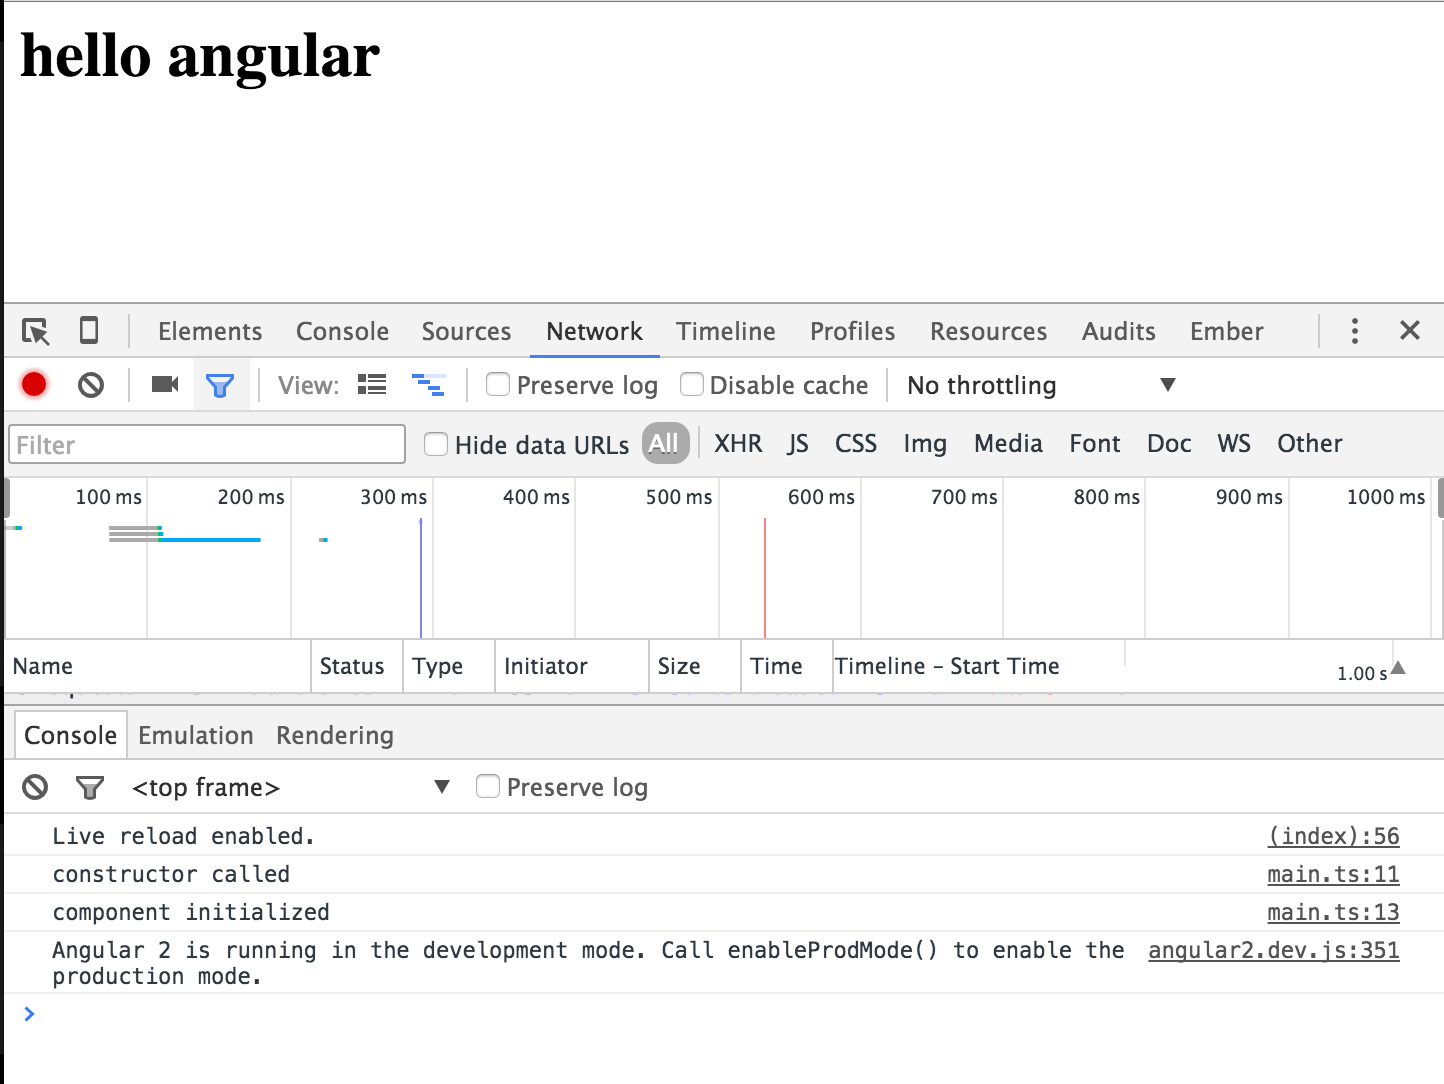
\includegraphics{images/hello-angular.png}
\caption{Running a basic component in the browser}
\end{figure}

\subsection{Dependency Injection}\label{dependency-injection}

Dependency Injection is a coding pattern in which a class receives its
dependencies from external sources rather than creating them itself. In
order to achieve Dependency Injection we need a Dependency
InjectionFramework to handle the dependencies for us. Using a DI
framework, you simply ask for a class from the injector instead of
worrying about the dependencies inside the class itself.

Angular has a standalone module that handles Dependency Injection. This
framework can also be used in non-Angular applications to handle
Dependency Injection.

\subsection{Services and Providers}\label{services-and-providers}

\begin{itemize}
\item
  A service is nothing more than a class in Angular 2. It remains
  nothing more than a class until we register it with the Angular
  injector.
\item
  When you bootstrap your app, Angular creates an injector on the fly
  that can inject services and other dependencies throughout the app.
\item
  You can register the service or the dependencies during when
  bootstrapping the app or when defining a component.
\item
  If you have a class called \texttt{MyService}, you can register it
  with the Injector and then you can inject it everywhere:

\begin{Shaded}
\begin{Highlighting}[numbers=left,,]
\FunctionTok{bootstrap}\NormalTok{(App, [MyService]); }\CommentTok{// second param is an array of providers}
\end{Highlighting}
\end{Shaded}
\item
  Providers is a way to specify what services are available inside the
  component in a hierarchical fashion.
\item
  A provider can be a class, a value or a factory.
\item
  Providers create the instances of the things that we ask the injector
  to inject.
\item
  \texttt{{[}SomeService{]};} is short for
  \texttt{{[}provide(SomeService,\ \{useClass:SomeService\}){]};} where
  the first param is the token, and the second is the definition object.
\item
  A simple object can be passed to the Injector to create a Value
  Provider:

\begin{Shaded}
\begin{Highlighting}[numbers=left,,]
\FunctionTok{beforeEachProviders}\NormalTok{(() => \{}
  \NormalTok{let someService = \{ getData: () => [] \};}
  \CommentTok{// using `useValue` instead of `useClass`}
  \KeywordTok{return} \NormalTok{[ }\FunctionTok{provide}\NormalTok{(SomeSvc, \{useValue: someService\}) ];}
\NormalTok{\});}
\end{Highlighting}
\end{Shaded}
\item
  You can also use a factory as a provider.
\item
  You can use a factory function that creates a properly configured
  Service:

\begin{Shaded}
\begin{Highlighting}[numbers=left,,]
\NormalTok{let myServiceFactory = (dx: DepX, dy: DepY) => \{}
  \KeywordTok{return} \KeywordTok{new} \FunctionTok{MyService}\NormalTok{(dx, dy.}\FunctionTok{value}\NormalTok{);}
\NormalTok{\}}

\CommentTok{// provider definition object.}
\NormalTok{let myServiceDefinition = \{}
   \NormalTok{useFactory: myServiceFactory,}
   \NormalTok{deps: [DepX, DepY]}
\NormalTok{\};}

\CommentTok{// create provider and bootstrap}
\NormalTok{let myServiceProvider = }\FunctionTok{provide}\NormalTok{(MyService, myServiceDefinition);}
\FunctionTok{bootstrap}\NormalTok{(AppComponent, [myServiceProvider, DepX, DepY]);}
\end{Highlighting}
\end{Shaded}
\item
  Defining object dependencies is simple. You can make a plain
  JavaScript object available for injection using a string-based token
  and the \texttt{@Inject} decorator:

\begin{Shaded}
\begin{Highlighting}[numbers=left,,]
\NormalTok{var myObj = \{\};}

\FunctionTok{bootstrap}\NormalTok{(AppComponent, [}
  \FunctionTok{provide}\NormalTok{('coolObjToken', \{useValue: myObj\})}
\NormalTok{]);}

\CommentTok{// and you can inject it to a component}

\KeywordTok{import} \NormalTok{\{Inject\} from 'angular2/core'}
\FunctionTok{constructor}\NormalTok{(dx: DepX, }\FunctionTok{@Inject}\NormalTok{('coolObjToken') config)}
\end{Highlighting}
\end{Shaded}
\end{itemize}

\end{document}
